\documentclass[10pt,letterpaper]{article}
\usepackage[top=0.85in,left=2.75in,footskip=0.75in,marginparwidth=2in]{geometry}
\usepackage{listings}

% use Unicode characters - try changing the option if you run into troubles with special characters (e.g. umlauts)

\usepackage[utf8]{inputenc}


% clean citations
\usepackage{cite}

% hyperref makes references clicky. use \url{www.example.com} or \href{www.example.com}{description} to add a clicky url
\usepackage{nameref,hyperref}

% line numbers
\usepackage[right]{lineno}

% improves typesetting in LaTeX
\usepackage{microtype}
\DisableLigatures[f]{encoding = *, family = * }

% text layout - change as needed
\raggedright
\setlength{\parindent}{0.5cm}
\textwidth 5.25in
\textheight 8.75in

% use adjustwidth environment to exceed text width (see examples in text)
\usepackage{changepage}

% adjust caption style

% remove brackets from references
\makeatletter
\renewcommand{\@biblabel}[1]{\quad#1.}
\makeatother

% headrule, footrule and page numbers
\usepackage{lastpage,fancyhdr,graphicx}
\usepackage{epstopdf}
\pagestyle{myheadings}
\pagestyle{fancy}
\fancyhf{}
\rfoot{\thepage/\pageref{LastPage}}
\renewcommand{\footrule}{\hrule height 2pt \vspace{2mm}}
\fancyheadoffset[L]{2.25in}
\fancyfootoffset[L]{2.25in}

% use \textcolor{color}{text} for colored text (e.g. highlight to-do areas)
\usepackage{color}

% define custom colors (this one is for figure captions)
\definecolor{Gray}{gray}{.25}

% this is required to include graphics
\usepackage{graphicx}

% use if you want to put caption to the side of the figure - see example in text
\usepackage{sidecap}

% use for have text wrap around figures
\usepackage{wrapfig}
\usepackage[pscoord]{eso-pic}
\usepackage[fulladjust]{marginnote}
\reversemarginpar

% document begins here
\begin{document}
\vspace*{0.35in}

% title goes here:
\begin{flushleft}
{\Large
  \textbf\newline{pyranges: efficient comparisons of genomic intervals in Python}
  % and arithmetic run length-encoding
}
\newline
% authors go here:
\\
Endre Bakken Stovner\textsuperscript{1},
Pål Sætrom\textsuperscript{1, 2},
\\
\bf{1} Department of
  Computer Science, Norwegian University
  of Science and Technology, Trondheim, 7013, Norway
\\
\bf{2} Department of Clinical and Molecular Medicine, Norwegian
  University of Science and Technology, Trondheim, 7013, Norway
\\
\bf{3} Bioinformatics Core Facility, Norwegian University of Science and
Technology, Trondheim, 7013, Norway
\\
\bf{4} K.G. Jebsen Center for Genetic Epidemiology, Department of Public Health
and Nursing, Norwegian University of Science and Technology, Trondheim, Norway
\\
\bigskip
* endrebak85@gmail.com

\end{flushleft}

\section*{Abstract}

\textbf{Summary:} Complex genomic analyses are carried out by a sequence of
simple operations like intersection, overlap and nearest. So a toolbox of these
operations enables a wide range of analyses to be performed. To this end, we
have written PyRanges, a datastructure for representing and manipulating genomic
intervals and their associated data in Python. It is directly compatible with
Python's wealth of data science libraries. Our benchmarks show that on average
PyRanges is 30 times faster and uses 50 percent of the memory of the popular R
GenomicRanges library.

\textbf{Availability and Implementation:} PyRanges is available open-source under
the MIT license at https://github.com/endrebak/pyranges and documentation exists
at https://endrebak.github.io/pyranges/

\textbf{Contact:} endrebak85@gmail.com

\section*{Introduction}

Comparing sets of intervals ('genome arithmetic') is a fundamental task in
genomics, and a few basic operations allow for answering many scientific
questions. As a simple example, to find which genes a transcription factor binds
to, the collection of intervals representing the positions of the genes and the
collection representing the aligned positions of the transcription factor can be
overlapped. The overlap operation takes two collections of intervals and reports
all intervals from the first collection which shares at least a part of its
position with an interval from the second. For the remainder of the
transcription factor alignments which did not overlap any genes, one can use the
operation nearest to find the genes with the shortest nucleotide
distance to them. Of course, a complete genomic analysis will often require
additional custom manipulation of data, which can be achieved by programming.

Genomics datasets can be large - alignment files can contain hundreds of
millions of entries, which means that software for performing genome arithmetic
need to find a compact representation of the data and that the operations should
be fast, otherwise many problems become intractable due to the excessive time or
computational resources needed. Time usage can be reduced by leveraging a
beneficial property of genomic operations, namely that they are trivially
parallelizeable, as each operation is performed per chromosome. Using this fact
genomic software can produce a speedup equal to the time it takes to run the
code on the longest chromosome (or even better, chromosome/strand pair). This
all means that genomic analyses are hard to write, as they require the
programmer to understand software parallelism and lower-level aspects of
programming to write operations with the desired efficiency.

Several toolboxes of genomic operations exist, both for the command line and
programming environments.

For the command line, the most used alternative is bedtools
\cite{doi:10.1093/bioinformatics/btq033}. It allows for performing operations on
common bioinformatics file formats, which means that each sequence of operations
starts and ends with I/O. It works by streaming the data and evicting it from
memory as soon as it is not needed anymore. There is also a wrapper for bedtools
which allows easy use from Python \cite{doi:10.1093/bioinformatics/btr539}.

Since comparing sets of intervals is a fundamental task, the datastructure
GenomicRanges\cite{10.1371/journal.pcbi.1003118} for representing and operating
on genomic intervals was invented. This datastructure stores collections of
intervals and their metadata as a 2D-table in memory, and allows for
manipulating them from the comfort of ones programming environment. Indeed, in
R, GenomicRanges is a foundational library, and a cornerstone of genomics
packages in the R BioConductor \cite{Gentleman2004} project. The new Julia
language \cite{doi:10.1137/141000671} also has a package for GenomicRanges
\cite{Haverty2017}.

Conspicuouly missing from the list of languages with a GenomicRanges
implementation is Python. The Python language is perhaps the most used in the
world\footnotemark, and extremely popular in data science and bioinformatics,
yet it lacks a GenomicRanges implementation. The PyRanges library remedies this
by providing an implementation which is at least an order of magnitude faster
and 50 percent more memory-efficient than the existing alternatives and is the
first multi-threaded genomic toolbox.

\footnotetext{TIOBE}

\section*{Library}

\subsection*{Design goals}

PyRanges is an implementation of the GenomicRanges datastructure for Python
guided by three principles:

\begin{itemize}
  \item speed and memory-efficiency
  \item ease of use
  \item interoperability with the Python data science stack
  \item effortless parallelism
\end{itemize}


\subsubsection*{Speed and memory-efficiency}

PyRanges needs to be fast an memory-efficient so that it makes even very large
genomic analyses feasible and that it can serve as building block for future
genomics libraries in Python.

\subsubsection*{Ease of use}

* avoid creating many new classes and methods

* use known Python syntax

*

\subsubsection*{Interoperability with the existing Python data science stack}

Python has a large ecosystem of libraries for performing statistics, machine
learning and visualization. All these are made for working on Numpy arrays (or
their convenience wrappers Pandas Series/DataFrames) so by using these data
types to represent data, we enable a large number of statistical methods to be
used for analysing and manipulating PyRanges. Furthermore, this helps ease of
use as known methods can be used to manipulate PyRanges instead of having to
learn new syntax. Lastly, as Pandas is a continually developed library,
improvements to the Pandas library in speed and memory will benefit PyRanges.

\subsubsection*{Effortless parallelism}

All methods on PyRanges should be able to run in parallel. As genomes are made
up of collections of discrete data called chromosomes, and the operations for
each chromosome is independent of that of the others, it is possible to run all
operations in parallel. For this reason PyRanges should have a framework for
running functions in parallel per chromosome, so that users and developers can
write the code that should run in parallel per chromosome and have PyRanges
apply it in parallel for them.

\subsection*{Description}

The main feature of the PyRanges library is the PyRanges datastructure, a
2D-table where each row represents an interval, and the columns each describe
part of the location (chromosome, start position, end position, and optionally,
strand) or metadata (name, score, exon number or any arbitrary value desired by
the user).

PyRanges objects are instantiated by creating them from regular Python objects,
Pandas Dataframes or reading common bioinformatics file formats such as bed, bam
or GTF/GFF.

The library provides operations for modifying single PyRanges and for comparing
pairs of PyRanges (listed in table\ref{tab1} and table\ref{tab2}, respectively).
It is not only the built-in functions which can be run in parallel, even
user-defined functions can take advantage of PyRanges framework for
multithreading, by using the apply or apply\_both functions (for manipulating
single PyRanges or comparing pairs of PyRanges, respectively).

Each binary operation supports the flags strandedness, which takes the values
'same', 'opposite' or False/None. These run the analyses on the same strand,
opposite strand or ignore strand information, respectively.

For methods used on single PyRanges, the flag strand exists, which is used to
indicate whether you want to run the operations per chromosome or per
chromosome/strand pair.

\begin{table}[!ht]
\begin{adjustwidth}{-1.5in}{0in}
\centering
\caption{{\bf PyRange Functionality.} Methods for manipulating/converting single PyRanges.}
\begin{tabular}{|l|l|l|l|l|l|l|}
\hline
  {\bf Method} & {\bf Purpose} \\ \hline
  Subset & Use Python's getitem operator to efficiently subset PyRanges \\ \hline
  Cluster & Merge the overlapping features in a PyRanges object \\ \hline
  Coverage & Create a dictionary of run length encodings (PyRles) from the PyRanges object \\ \hline
  Sort & Sort the dataframe on Starts and Ends (and/or any metadata columns) \\ \hline
  Tssify & Create a GRange for the area around the 5' end \\ \hline
  Tesify & Create a GRange for the area around the 3' end \\ \hline
  Slack & Extend the interval in the 5' and 3' ends \\ \hline
  As\_matrix & Return the PyRanges data as a Pandas Dataframe \\ \hline
  Apply & Apply a user-defined function to the PyRange \\ \hline
\end{tabular}
\label{tab1}
\end{adjustwidth}
\end{table}

\begin{table}[!ht]
\begin{adjustwidth}{-1.5in}{0in}
\centering
\caption{{\bf PyRange Functionality.} Methods available on PyRanges objects.}
\begin{tabular}{|l|l|l|l|l|l|l|}
\hline
  {\bf Method} & {\bf Purpose} \\ \hline
  Intersection & For each feature in self, keep those that overlap with intervals in other \footnotemark \\ \hline
  Set Intersection & Treat the intervals in each PyRanges as a set and find the intersection \footnotemark \\ \hline
  Overlap & Keep each feature in self that overlaps with at least one in other \\ \hline
  Set Union & Treat the intervals in each PyRanges as a set and find the union \\ \hline
  Subtract & For each feature in self, keep those parts that do not overlap with any feature in other \\ \hline
  Set Subtract & Treat the intervals in each PyRanges as a set and subtract other from self \\ \hline
  Nearest & For each feature in self, find the nearest in other \\ \hline
  Apply\_both & Apply a user-defined function for comparing two PyRanges \\ \hline
\end{tabular}
\label{tab2}
\end{adjustwidth}
\end{table}
\footnotetext{Like bedtools intersect}
\footnotetext{Like BioConductor GenomicRanges intersect}

\begin{table}[!ht]
\begin{adjustwidth}{-1.5in}{0in}
\centering
\caption{{\bf PyRanges I/O Functionality.}}
\begin{tabular}{|l|l|l|l|l|l|l|}
\hline
  {\bf Method} & {\bf Purpose} \\ \hline
  read\_bed & Read a bed file, turning it into a PyRanges object\\ \hline
  read\_bam & Read a bam file, turning it into a PyRanges object\\ \hline
  read\_gtf & Read a GTF/GFF file, turning it into a PyRanges object\\ \hline
  to\_csv & Write a PyRanges object to a tabular file \\ \hline
\end{tabular}
\label{tab3}
\end{adjustwidth}
\end{table}

\subsection*{Run Length Encoding library}

Additionally, PyRanges provides a run-length encoding (RLE) datastructure for
compactly representing the coverage (or any nucleotide-associated score)
associated with one or more PyRanges. A run length encoding is a way to compress
continuous stretches of data to two values, namely a run length and a value. As
an example, 11100111100 can be represented as [3, 2, 4, 2], [1, 0, 1, 0]. The
arithmetic operations +, -, / and * are implemented for the RLEs, all producing
new RLEs. This enables nucleotide-level computations and comparisons of coverage
or scores from pairs of interval collections, even though they cover genomes
spanning billions of nucleotides.

The class PyRles allows one to conveniently compare collections of Rles
representing genomes. Using these arithmetic operations can be performed per
chromosome (or each chromosome/strand pair), by simply calling any arithmetic
operation (e.g. +) on the two PyRles.

\subsection*{Nested Containment List}

PyRanges also provides a modified implementation of the Nested Containment List.
This library is especially made for PyRanges, but written to allow independent
use and made available to the general public. It has the neat property that it
takes Numpy arrays and Pandas Series as input both when creating the NCLS and
when executing queries. Numpy arrays and Pandas Series are both stored
contiguously in memory with low-level datatypes, which means that both NCLS
creation and overlap queries happen at the speed of highly optimized C, even
though each operation is performed with one single line of Python code.

\section*{Example usage}

blablabla

\section*{Implementation}

\subsection*{PyRanges}

To store the intervals and associated metadata, Pandas dataframes are used.
Pandas dataframes are 2D tables where both axes are labeled. Each column in a
Pandas Dataframe is stored as a contiguous array of a low-level datatype (i.e.
int, uint32, float64) or pointers to Python objects.

The location-related aspects are compactly represented, using 32-bit unsigned
integers for the starts and ends, an 8-bit int categorical for the strand and an
8-bit int categorical for the chromosome (or 16-bit, if the number of
chromosomes is above 256). There is also a flag which allows creating extended
PyRanges, where the starts and ends are stored as 64-bit ints). The data
associated with each chromosome/strand pair are kept in their own dataframe, so
that the table of genomic data does not need to be split or combined after
distributing the data to different cores for parallel processing (this division
is invisible to the end-user however).

Each row unique integer index. These found with NCLS...

Multithreading is achieved by using the Ray library to distribute jobs on
different cores for asynchronous computation \cite{}. How this is done...

\subsection*{PyRles}

Each run length encoding uses 64-bit integers to store the run lengths and
64-bit floats to store the associated values. The convenience class PyRles is
implemented as a simple Python class, where each RLE is stored in a dict.

\subsection*{Nested Containment List}

PyRanges uses the Nested Containment
List\cite{doi:10.1093/bioinformatics/btl647} (NCLS) for overlap operations. The
NCLS is a tree-like structure for performing interval queries. It works by
sorting an array of intervals into one main list and then (possibly) several
sublists, where each list upholds the property that no interval in the list is
purely contained in another. This allows for binary searches in each list, and
it has the nice property that as the first overlapping interval is found, the
rest can be retrieved by simple linear iteration.

The NCLS used for PyRanges is a modified version of the nclist written for the
now defunct PyGR library. The main changes are reducing the interval structure
to only contain a start, end and ID (thereby reducing the memory use by 40
percent), and implementing a 32 bit version, (thereby reducing the memory
consumption by another 50 percent). Furthermore, the NCLS has been augmented
with a collection of methods, which enables passing arrays of starts and ends to
query the NCLS completely in C.

\section*{Performance}

The PyRanges library has been extensively benchmarked for both speed and memory
use. In the below tests, unsorted files generated by bedtools random for hg38
were used. Unsorted data do not affect the runtime or memory-usage of
PyRanges/GenomicRanges, but makes some PyBedTools-operations slower and more
memory-consuming. But as sorting large amounts of data needs much time and
memory, it is not likely that a benchmark that included sorting the data then
running bedtools would lead to a more favorable benchmark. Note that as all
PyBedTools operations start with and and end with I/O, it is not possible
to measure the speed of the operations themselves.

\subsection*{Speed}


% \begin{figure}
% % the number in [] of wrapfigure is optional and gives the number of text lines that should be wrapped around the text. Adjust according to your figures height
% 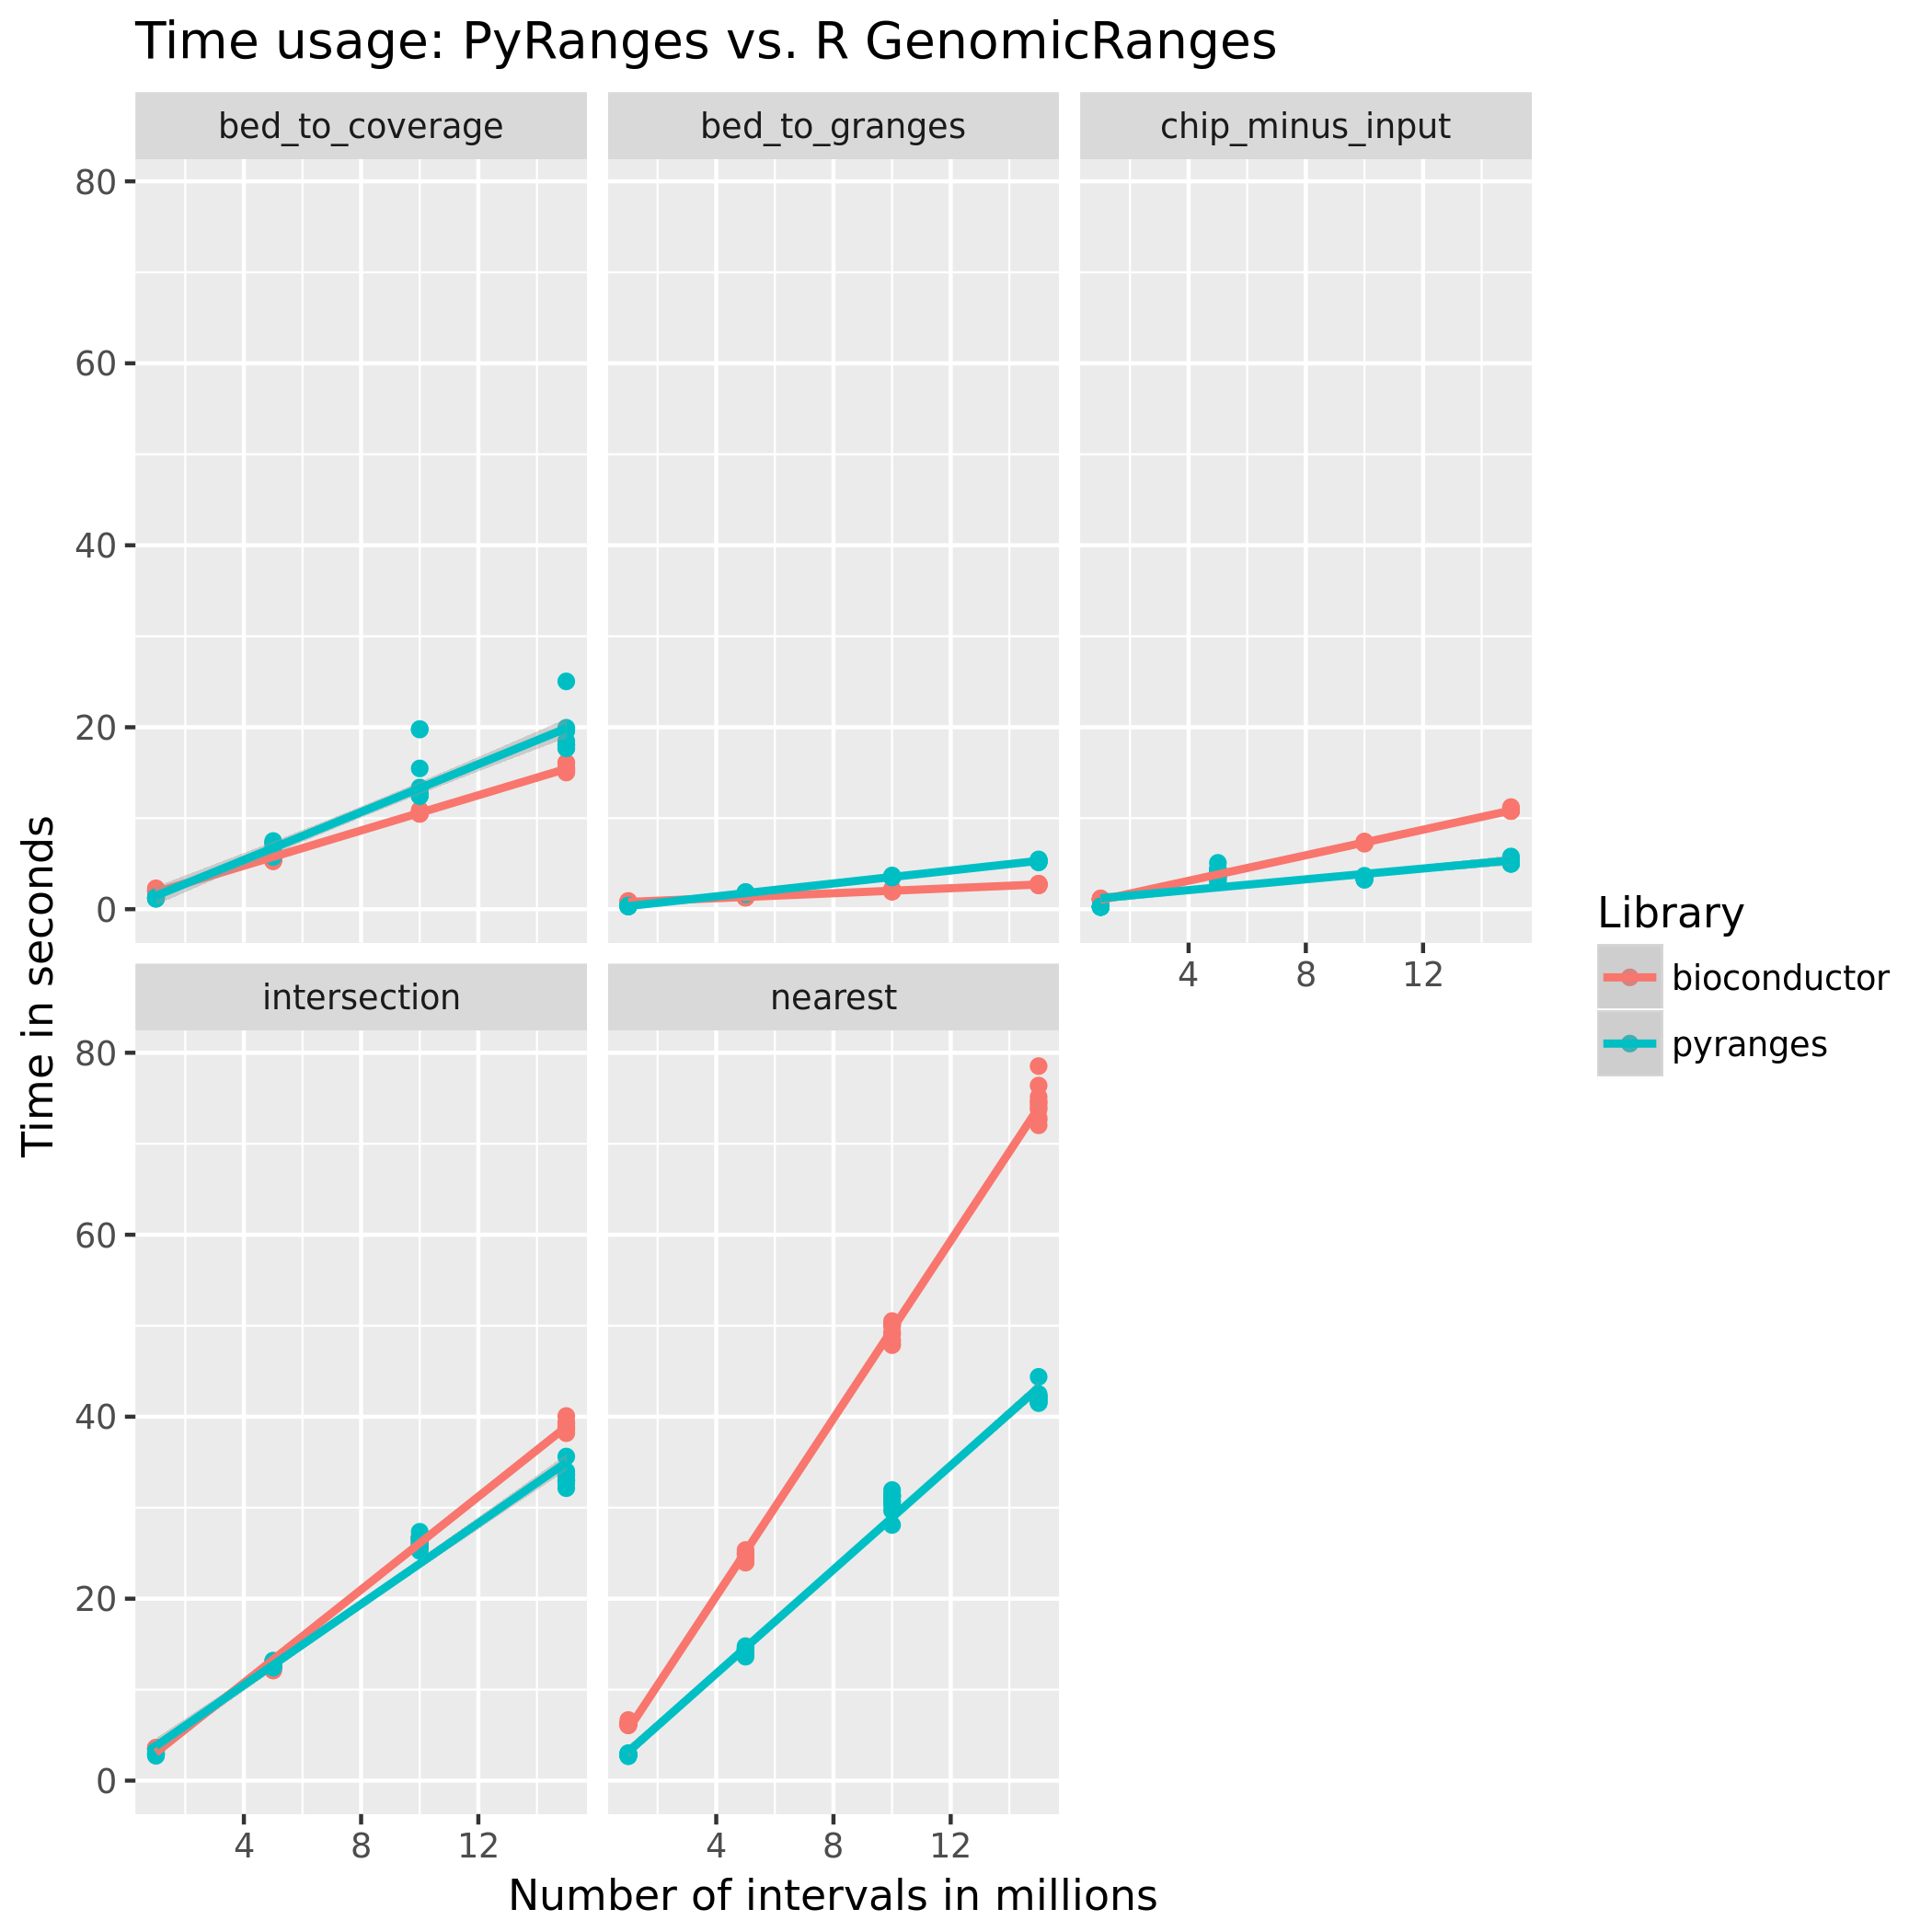
\includegraphics[width=1\textwidth]{graphs/time.pdf}
% % \captionsetup{labelformat=empty} % makes sure dummy caption is blank
% \caption{Time in seconds: PyRanges vs. GenomicRanges} % add dummy caption - otherwise \label won't work and figure numbering will not count up
% \label{fig1} % use \ref{fig1} to reference to this figure
% \end{figure} % avoid blank space here

\subsection*{Memory usage}

Memory usage of the PyRanges library was tested using the benchmarking
capabilities of Snakemake \cite{doi:10.1093/bioinformatics/bty350}. It works by
polling the running process.

% For most functionality, PyRanges uses a bit less memory than GenomicRanges. The
% only cases where PyRanges uses more memory is for rle arithmetic and nearest,
% where PyRanges leverages this memory to make the operations much faster
% than R GenomicRanges. There is some variability in the memory usage, which is to
% be expected for garbage collected languages. We see that pybedtools is extremely
% memory-efficient for many operations.

% \begin{figure}
% % the number in [] of wrapfigure is optional and gives the number of text lines that should be wrapped around the text. Adjust according to your figures height
% 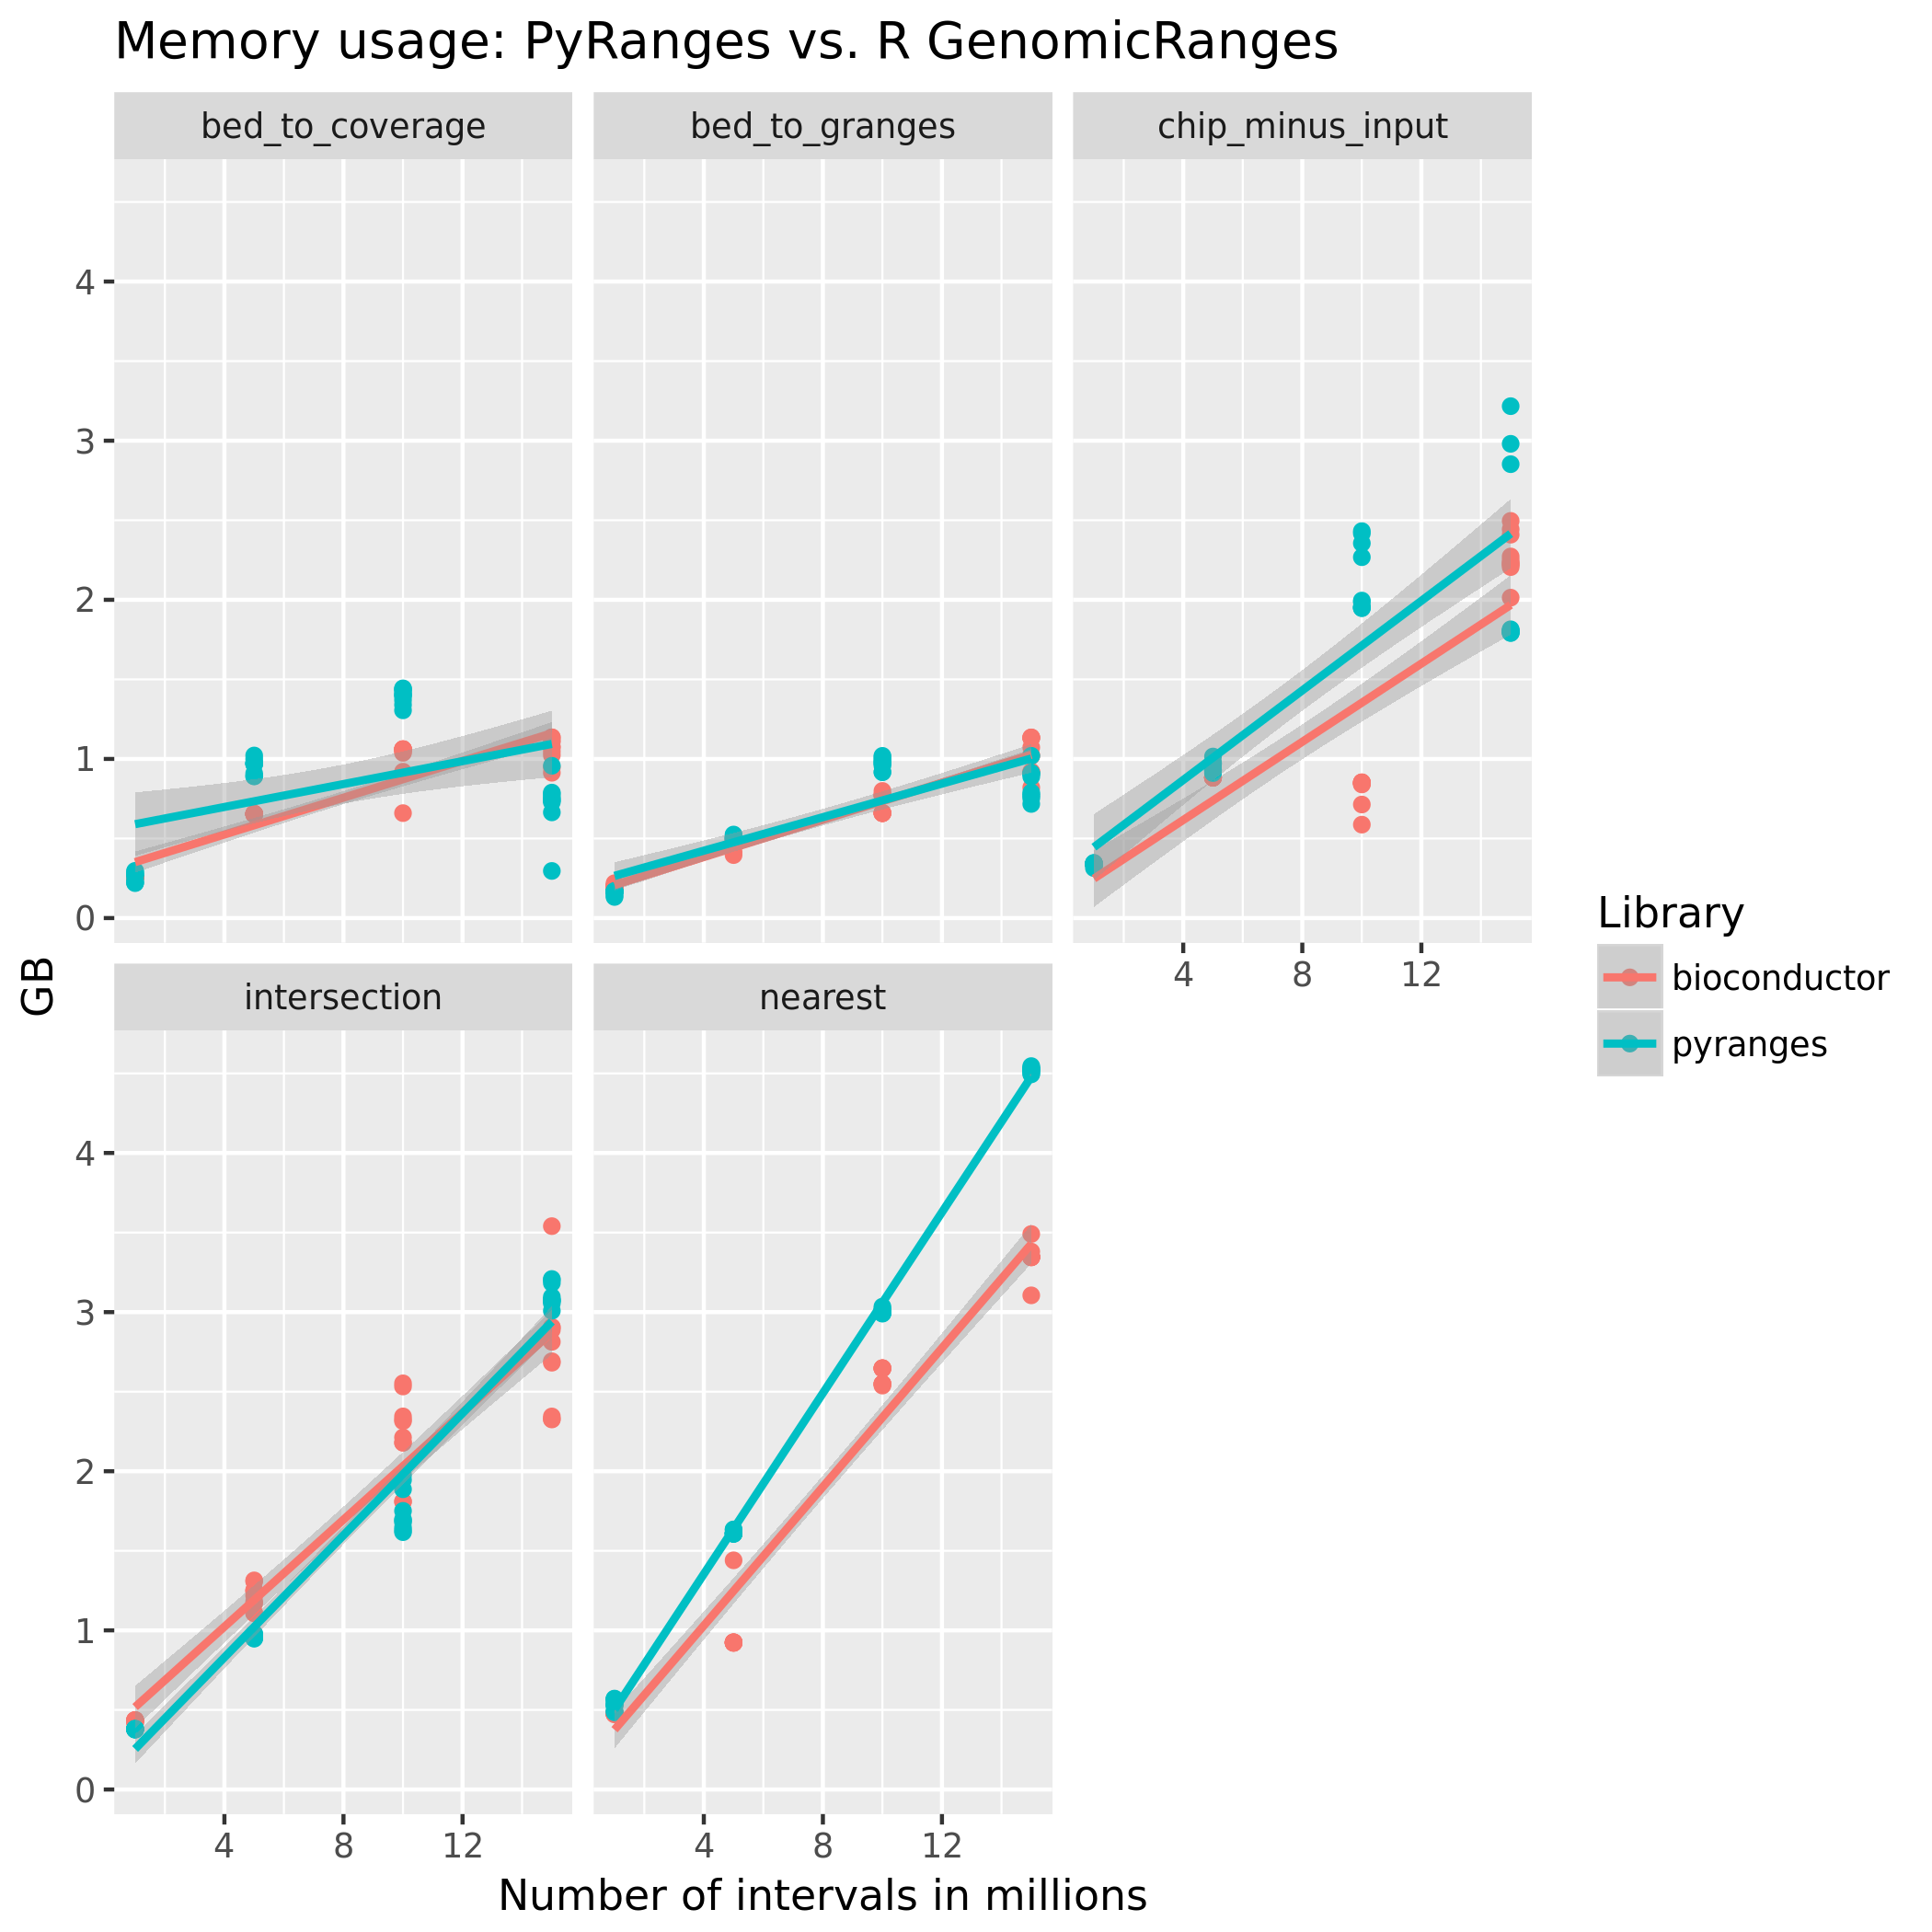
\includegraphics[width=1\textwidth]{graphs/memory.pdf}
% % \captionsetup{labelformat=empty} % makes sure dummy caption is blank
% \caption{Memory usage in GigaBytes: PyRanges vs GenomicRanges} % add dummy caption - otherwise \label won't work and figure numbering will not count up
% \label{fig2} % use \ref{fig1} to reference to this figure
% \end{figure} % avoid blank space here

\section*{Testing}

PyRanges has an extensive suite of tests written using the testing library
Hypothesis. This is a framework for genarating tests using the computer, so that
a much more thorough exercising of the code is possible. This is done using a
method called property based testing (PBT), which works by having the computer
generate random tests data according to some specification and then ensuring the
the output preserves some known invariant (e.g. that the square of an
non-imaginary number is positive.)

Two advantages of PBT is that an infinite number of tests can in principle be
generated and that these will include test cases exercising hairy edge-case
functionality which humans would likely not think of. The downside of PBT is
that you usually cannot ensure that the function produces the correct result in
each case, only that some invariant holds.

But in our case, as there exist mature and proven libraries that do the same
thing as our code (Bedtools for the PyRanges functionality and S4Vectors for the
PyRles) we can use these as "oracles" and actually test that our functions
produce the desired result.

\section*{Discussion}

\subsection*{PyRanges vs. R GenomicRanges}

PyRanges is a reimplementation of R GenomicRanges for Python. In addition to the
previously discussed speed and memory improvements, PyRanges is implemented with
a focus on user friendliness. This has resulted in a much simplified
user-experience than R GenomicRanges, visible in the following ways:

\begin{itemize}
  \item It is easier to create a PyRanges (can read as dataframe and turn into GRange)
  \item Different methods for accesing/setting locattion and metadata
  \item subsetting PyRanges takes much less code than subsetting GenomicRanges
  \item the PyRanges API is much more streamlined
\end{itemize}

Since PyRanges has a framework for parallelism, can be used by libraries built
on top of it so whole ecosystem has 'free' multithreading.

Since Pandas-operations work on genomicranges, can use skills already know or
learn useful skills while operating on PyRanges. Furthermore, as Pandas
improved/extended so are PyRanges.

Do fewer R GenomicRanges operations retain metadata?

Switching out multithreaded backend also easy.

and seamless integration with the Python data
science ecosystem

\subsection*{Comparison with bedtools/pybedtools}

PyBedtools is a wrapper for using bedtools in Python. However, its dependence on
bedtools limits it flexibility and speed in many ways.

\subsubsection*{PyRanges vs. bedtools}

Some limitations that are inherent in bedtools that does not exist in PyRanges
is that

\begin{enumerate}
  \item bedtools needs the data to adhere to predefined bioinformatics-formats
    for it to understand them
  \item data is streamed, not stored in memory
  \item some operations require pre-sorted data
  \item not possible to subset the data
\end{enumerate}

An example of rigid format requirements leading to hard to understand and debug
behavior in bedtools is that you cannot run stranded operations on files where
strand is not the sixth column, since the bed-format definition says that strand
is the sixth column. Instead bedtools runs the operation without taking strand
into consideration, without any warning or error-messages, silently producing
the wrong result. In comparison, PyRanges can have arbitrarily many or few
columns in any order, which means that it can operate on any tabular
bioinformatics-file, as long as these contain one interval per row. This is a
tremendous boon for bioinformatics where there is a profilation of new, ad-hoc
or slightly modified file formats.

Bedtools uses the efficient fjoin-algorithm (O(n*k) speed/O(1) memory algorithm)
to find overlaps when the input-data is sorted. However, as this operation does
not produce sorted output, it means that in a sequence of steps, each step in a
pipeline needs to be followed by a sort operation for bedtools to retain its
efficiency. While PyRanges also requires sorting for all its overlap-based
operations, it already has the data in memory and only needs to sort the
intervals in the \textit{queried} dataset. Furthermore, PyRanges only needs to
sort the coordinates themselves (structs of three 32- or 64-bit integers -
start, end and index), while bedtools needs to sort the order of the
entries in the bed/bam/vcf/GFF or GTF-files themselves, which is orders of
magnitude more expensive.

Bedtools use of streaming can lead to annoying behavior as an out of order entry
might not be discovered until the end of a (possibly long-running) operation,
but which would then make bedtools abort.

\subsubsection*{PyRanges vs. PyBedtools}

PyBedtools gives access to bedtools from the Python programming-environment. It
does not really extend the capabilities of bedtools, but rather makes it more
convenient to use by allowing the user to operate on streams of data using
Python, instead of UNIX tools. As bedtools does not keep data in memory, one
needs to operate on streams. Pybedtools allows this streaming by turning each
entry into a Python-object for manipulations and then converting these back to a
textual format for the output stream. This is very slow. Compare this with
PyRanges which operates on contiguously arranged low-level datatypes at C-level
speed.
% TODO: can one access custom fields?

A further limitation of this streaming approach is that none of Pythons vast
number of high-performance scientific libraries can be used on the data, as
these operate on contiguous arrays, not single entries of custom datatypes.

\subsection*{PyRles vs. S4Vectors}


\subsection*{NCLS vs. bisection}

\section*{Conclusion}



\bibliography{library}

\bibliographystyle{abbrv}

\end{document}


% \subsection*{Advantages}

% In contrast to PyRanges, which stores the data in memory, PyBedtools uses disk
% space for storing temporary results, which requires additional resource
% management by users and can lead to resource leaks; e.g. if the process calling
% PyBedtools is killed.

% PyBedtools: rigid in input format. If one operation merges reads and does not
% preserve all columns, then the file is not usable in further operations with
% bedtools.

% To make it go fast, need to sort. If already sorted, this is a waste of time.
% Often a bother; need to keep two copies of same file.

% Cannot do region-based lookups in bedfile easily.



% \section*{Example Usage}

% \begin{adjustwidth}{-2in}{0in}
% \begin{flushright}
% \begin{lstlisting}[language=Python, linewidth=30cm, basicstyle=\small]
%   import pyranges as pr
%   from pyranges import PyRanges

%   > gr1 = pr.read_bed('f1.bed')

%   +--------------+---------+-------+--------+---------+----------+
%   | Chromosome   |   Start |   End | Name   |   Score | Strand   |
%   |--------------+---------+-------+--------+---------+----------|
%   | chr1         |       3 |     6 | h      |       0 | +        |
%   | chr1         |       5 |     7 | h      |       0 | -        |
%   | chr1         |       8 |     9 | h      |       0 | +        |
%   +--------------+---------+-------+--------+---------+----------+
%   PyRanges object has 3 sequences from 1 chromosomes.

%   > gr2 = pr.read_bed('f2.bed')

%   +--------------+---------+-------+--------+---------+----------+
%   | Chromosome   |   Start |   End | Name   |   Score | Strand   |
%   |--------------+---------+-------+--------+---------+----------|
%   | chr1         |       1 |     2 | f      |       0 | +        |
%   | chr1         |       6 |     7 | f      |       0 | -        |
%   +--------------+---------+-------+--------+---------+----------+
%   PyRanges object has 2 sequences from 1 chromosomes.

%   > n = gr1.nearest(gr2, strandedness="opposite", overlapping=False, suffix='_')

%   # The PyRanges data can be accessed with .df
%   > n.df[["Chromosome", "Start", "End", "Strand", "Start_", "End_", "Strand_", "Distance"]]

%     Chromosome  Start  End Strand  Start_  End_ Strand_  Distance
%   0       chr1      3    6      +       6     7       -         1
%   1       chr1      8    9      +       6     7       -         2
%   2       chr1      5    7      -       1     2       +         4

%   # Easily create new PyRanges from a df

%   > PyRanges(n.df[["Chromosome", "Start", "End", "Strand", "Start_", "End_", "Strand_", "Distance"]])

%   +--------------+---------+-------+----------+----------+--------+-----------+------------+
%   | Chromosome   |   Start |   End | Strand   |   Start_ |   End_ | Strand_   |   Distance |
%   |--------------+---------+-------+----------+----------+--------+-----------+------------|
%   | chr1         |       3 |     6 | +        |        6 |      7 | -         |          1 |
%   | chr1         |       8 |     9 | +        |        6 |      7 | -         |          2 |
%   | chr1         |       5 |     7 | -        |        1 |      2 | +         |          4 |
%   +--------------+---------+-------+----------+----------+--------+-----------+------------+
%   PyRanges object has 3 sequences from 1 chromosomes.

%   > gr1.intersection(gr2)

%   +--------------+---------+-------+--------+---------+----------+
%   | Chromosome   |   Start |   End | Name   |   Score | Strand   |
%   |--------------+---------+-------+--------+---------+----------|
%   | chr1         |       6 |     7 | h      |       0 | -        |
%   +--------------+---------+-------+--------+---------+----------+
%   PyRanges object has 1 sequences from 1 chromosomes.

%   > c = gr1.cluster()
%   > c

%   +--------------+---------+-------+
%   | Chromosome   |   Start |   End |
%   |--------------+---------+-------|
%   | chr1         |       3 |     7 |
%   | chr1         |       8 |     9 |
%   +--------------+---------+-------+
%   PyRanges object has 2 sequences from 1 chromosomes.

%   > c.df.insert(3, 'ID', ["A", "B"])
%   > c

%   +--------------+---------+-------+------+
%   | Chromosome   |   Start |   End | ID   |
%   |--------------+---------+-------+------|
%   | chr1         |       3 |     7 | A    |
%   | chr1         |       8 |     9 | B    |
%   +--------------+---------+-------+------+
%   PyRanges object has 2 sequences from 1 chromosomes.

%   > cv1 = gr1.coverage(strand=True)
%   > cv1

%   chr1 +
%   --
%   +--------+-----+-----+-----+-----+
%   | Runs   |   3 |   3 |   2 |   1 |
%   |--------+-----+-----+-----+-----|
%   | Values |   0 |   1 |   0 |   1 |
%   +--------+-----+-----+-----+-----+
%   Rle of length 9 containing 4 elements

%   chr1 -
%   --
%   +--------+-----+-----+
%   | Runs   |   5 |   2 |
%   |--------+-----+-----|
%   | Values |   0 |   1 |
%   +--------+-----+-----+
%   Rle of length 7 containing 2 elements
%   PyRles object with 2 chromosomes/strand pairs.

%   > cv2 = gr2.coverage(strand=True)
%   > cv2

%   chr1 +
%   --
%   +--------+-----+-----+
%   | Runs   |   1 |   1 |
%   |--------+-----+-----|
%   | Values |   0 |   1 |
%   +--------+-----+-----+
%   Rle of length 2 containing 2 elements

%   chr1 -
%   --
%   +--------+-----+-----+
%   | Runs   |   6 |   1 |
%   |--------+-----+-----|
%   | Values |   0 |   1 |
%   +--------+-----+-----+
%   Rle of length 7 containing 2 elements
%   PyRles object with 2 chromosomes/strand pairs.

%   > cv1 - cv2

%     chr1 +
%   --
%   +--------+-----+-----+-----+-----+-----+-----+
%   | Runs   |   1 |   1 |   1 |   3 |   2 |   1 |
%   |--------+-----+-----+-----+-----+-----+-----|
%   | Values |   0 |  -1 |   0 |   1 |   0 |   1 |
%   +--------+-----+-----+-----+-----+-----+-----+
%   Rle of length 9 containing 6 elements

%   chr1 -
%   --
%   +--------+-----+-----+-----+
%   | Runs   |   5 |   1 |   1 |
%   |--------+-----+-----+-----|
%   | Values |   0 |   1 |   0 |
%   +--------+-----+-----+-----+
%   Rle of length 7 containing 3 elements
%   PyRles object with 2 chromosomes/strand pairs.

% \end{lstlisting}
% \end{flushright}

% \end{adjustwidth}